\documentclass[presentation]{beamer}
\mode<presentation>{\usetheme{AMSBolognaFCrev}}

\usepackage[utf8]{inputenc}
\usepackage[T1]{fontenc}
\usepackage{booktabs}
\usepackage{array}
\usepackage{colortbl}
\usepackage{tikz}
\usepackage[ddmmyyyy]{datetime}
\usepackage[export]{adjustbox}
\usetikzlibrary{arrows.meta,positioning,shapes.geometric}

\renewcommand{\dateseparator}{/}
\newcommand{\sectiontitleframe}[1]{
\begin{frame}[plain,c]
\begin{center}
{\usebeamerfont{title}\usebeamercolor[fg]{title}#1}
\end{center}
\end{frame}
}

\title[Lesson 2]{Cryptographic Foundations for Healthcare Systems}
\institute[Data Privacy and Security]{Healthcare Data Privacy and Security}
\author[\sspeaker{G. Pisano}]{\speaker{Giuseppe Pisano} \\\href{mailto:g.pisano@unibo.it}{g.pisano@unibo.it}}
\date[August, 2026]{August, 2026}
%
\titlegraphic{
%\vspace{0.2cm}
\begin{center}
    
\includegraphics[width=0.35\textwidth, valign=c]{logos/intestazione.png}
    
\includegraphics[width=0.16\textwidth, valign=c]{logos/unibo_logo_2.png}
    
\includegraphics[width=0.11\textwidth, valign=c]{logos/makeni_logo_2.png}
    
\includegraphics[width=0.20\textwidth, valign=c]{logos/cuamm_logo_png.png}
\end{center}
\centering
\tiny{S.K.I.L.L.E.D --- AID013244/04/2\\Strategic Knowledge and Inclusive Lifelong Learning in the health sector for youth Employability and Development}
}

\begin{document}

\setbeamertemplate{frametitle}
{
    \nointerlineskip
    \begin{beamercolorbox}[sep=0.3cm,ht=2.2em,wd=\paperwidth]{frametitle}
        \vbox{}\vskip-2ex%
        \strut\insertframetitle\hfill\raisebox{-0.2\height}{
\includegraphics[width=2cm]{logos/cuamm_logo_png.png}}\strut
        \vskip-0.8ex%
    \end{beamercolorbox}
}

\begin{frame}[allowframebreaks]
\titlepage
\end{frame}

\begin{frame}[c,allowframebreaks]{Roadmap}
\tableofcontents[hideallsubsections]
\end{frame}

\begin{frame}[c]{How This Lesson Progresses}
\begin{block}{Learning path}
We move from \textbf{why cryptography is needed}, to \textbf{symmetric algorithms}, then to
\textbf{blocks, streams, and modes}. After that we add \textbf{integrity}, \textbf{public-key
cryptography}, certificates, envelopes, key management, and randomness.
\end{block}

\begin{exampleblock}{Hospital storyline}
We continue with St. Isidore Hospital. Encryption will protect EHR records, lab messages,
pharmacy orders, backups, remote access, and communication with external providers.
\end{exampleblock}
\end{frame}

\begin{frame}[c]{What This Lesson Prepares}
\begin{block}{Connection to later topics}
This lesson gives the vocabulary needed to understand TLS, VPNs, secure email, authentication,
digital signatures, and key-management policies.
\end{block}

\begin{itemize}
    \item \textbf{Networking}: where encrypted channels are established.
    \item \textbf{Access management}: how keys, passwords, and identities are protected.
    \item \textbf{GDPR}: why confidentiality, integrity, and breach prevention matter for personal data.
\end{itemize}
\end{frame}

\section{Cryptographic Foundations}
\sectiontitleframe{Cryptographic Foundations}

\begin{frame}[c]{Section Context: Cryptographic Foundations}
\begin{block}{What we are talking about}
Cryptography transforms information so that only authorised parties can read it, verify it, or
trust where it came from. We start with the basic ideas before looking at specific families of
algorithms.
\end{block}

\begin{exampleblock}{Hospital lens}
At St. Isidore, cryptography protects a lab result while it travels, a backup while it is stored,
and a prescription order while the pharmacy verifies who sent it.
\end{exampleblock}
\end{frame}

\begin{frame}[c]{Notebook: Classical Encryption}
\begin{block}{Practical example}
Open \texttt{lesson-02/examples/01\_classical\_caesar\_cipher.ipynb} after the Caesar cipher slides.
\end{block}

\begin{exampleblock}{What students should notice}
The notebook encrypts a hospital message, then breaks it by trying shifts and observing letter
patterns. The point is not that Caesar is useful; the point is that \textbf{patterns survive weak
encryption}.
\end{exampleblock}
\end{frame}

\begin{frame}[c]{Kerckhoffs's Principle}
\begin{block}{Principle}
The security of a cryptosystem should depend on the secrecy of the \textbf{key}, not on the secrecy
of the \textbf{algorithm} \cite{kerckhoffs_1883}.
\end{block}

\begin{exampleblock}{Hospital example}
St. Isidore should not rely on a vendor's secret home-made encryption method. It should rely on
well-studied algorithms and protect the hospital's keys carefully.
\end{exampleblock}
\end{frame}

\begin{frame}[c]{What Cryptography Provides}
\begin{block}{Core services}
Cryptography can support \textbf{confidentiality}, \textbf{authentication}, \textbf{integrity}, and in some
systems \textbf{anonymity}.
\end{block}

\begin{itemize}
    \item \textbf{Confidentiality}: hiding content from unauthorised readers.
    \item \textbf{Authentication}: verifying identities or sources.
    \item \textbf{Integrity}: detecting unauthorised modification.
    \item \textbf{Anonymity}: reducing linkability to a person or communication path.
\end{itemize}
\end{frame}

\begin{frame}[c]{Healthcare Example: One Lab Result}
\begin{exampleblock}{Hospital example}
A potassium result moves from the laboratory system to the EHR. Cryptography can keep the value
private, prove it came from the lab, detect changes, and help prevent replay of an old result.
\end{exampleblock}

\begin{block}{Takeaway}
Encryption is not only about secrecy. Clinical systems also need authenticity, integrity, freshness,
and correct ordering.
\end{block}
\end{frame}

\begin{frame}[c]{Encryption and Decryption}
\begin{block}{Concept}
\textbf{Encryption} transforms plaintext into ciphertext. \textbf{Decryption} transforms ciphertext
back into plaintext using the correct key.
\end{block}

\begin{exampleblock}{Hospital example}
Before sending a discharge letter to a referral clinic, the hospital encrypts it. If the message is
intercepted, the attacker sees ciphertext rather than patient data.
\end{exampleblock}
\end{frame}

\begin{frame}[c]{Scheme: Encryption Flow}
\begin{center}
\begin{adjustbox}{max width=\textwidth}
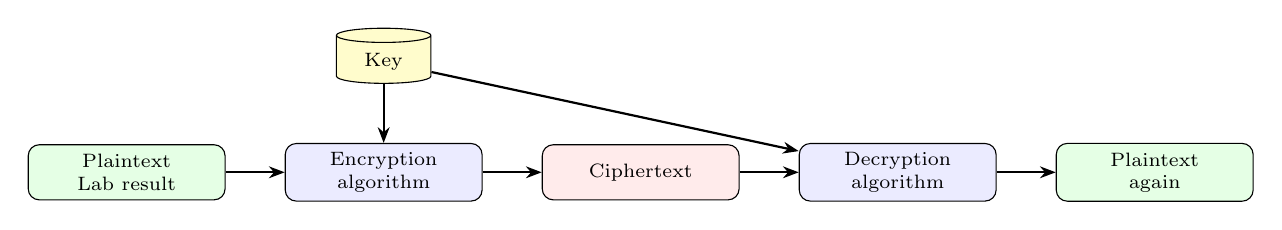
\begin{tikzpicture}[
    node distance=0.75cm,
    box/.style={draw, rounded corners, align=center, minimum width=2.5cm, minimum height=0.7cm, font=\scriptsize},
    key/.style={draw, cylinder, shape border rotate=90, aspect=0.25, align=center, minimum width=1.2cm, minimum height=0.7cm, font=\scriptsize, fill=yellow!20},
    link/.style={-{Stealth[length=2mm]}, thick}
]
\node[box, fill=green!10] (plain) {Plaintext\\Lab result};
\node[box, right=of plain, fill=blue!8] (enc) {Encryption\\algorithm};
\node[box, right=of enc, fill=red!8] (cipher) {Ciphertext};
\node[key, above=of enc] (key) {Key};
\node[box, right=of cipher, fill=blue!8] (dec) {Decryption\\algorithm};
\node[box, right=of dec, fill=green!10] (out) {Plaintext\\again};
\draw[link] (plain) -- (enc);
\draw[link] (enc) -- (cipher);
\draw[link] (cipher) -- (dec);
\draw[link] (dec) -- (out);
\draw[link] (key) -- (enc);
\draw[link] (key) -- (dec);
\end{tikzpicture}
\end{adjustbox}
\end{center}

\begin{block}{Reading the scheme}
The algorithm may be public. The key is the secret that controls who can decrypt.
\end{block}
\end{frame}

\begin{frame}[c]{Classical Ciphers}
\begin{block}{Concept}
Classical ciphers such as the Caesar cipher replace or move symbols according to a simple rule.
They are useful for teaching, but not for real security.
\end{block}

\begin{exampleblock}{Hospital example}
Changing every letter in a patient's name by three positions would not protect the record. Anyone
could reverse it once the pattern is recognised.
\end{exampleblock}
\end{frame}

\begin{frame}[c]{Why Simple Ciphers Fail}
\begin{block}{Concept}
Substitution and transposition ciphers preserve patterns. Attackers can use language statistics,
known formats, and repeated phrases to recover meaning.
\end{block}

\begin{exampleblock}{Hospital example}
Hospital messages often repeat phrases such as ``patient ID'', ``diagnosis'', or ``lab result''.
Repeated structure gives attackers clues if the cipher leaks patterns.
\end{exampleblock}
\end{frame}

\begin{frame}[c]{Recap: Cryptographic Foundations}
\begin{block}{Takeaways}
\begin{itemize}
    \item Cryptographic security should depend on protected keys, not secret algorithms.
    \item Encryption turns plaintext into ciphertext; decryption reverses it with the right key.
    \item Healthcare systems need secrecy, authenticity, integrity, and freshness.
    \item Simple historical ciphers fail because they leak patterns.
\end{itemize}
\end{block}
\end{frame}

\section{Symmetric Encryption}
\sectiontitleframe{Symmetric Encryption}

\begin{frame}[c]{Section Context: Symmetric Encryption}
\begin{block}{What we are talking about}
Symmetric encryption uses the \textbf{same secret key} for encryption and decryption. It is fast,
widely deployed, and central to protecting stored and transmitted healthcare data.
\end{block}

\begin{exampleblock}{Hospital lens}
When St. Isidore encrypts database backups or file transfers, it commonly uses symmetric
cryptography under the hood.
\end{exampleblock}
\end{frame}

\begin{frame}[c]{Symmetric Encryption}
\begin{block}{Concept}
In symmetric encryption, sender and receiver share one secret key. Anyone with the key can decrypt
the protected data.
\end{block}

\begin{exampleblock}{Hospital example}
The backup system encrypts nightly EHR backups with a hospital-controlled key. Recovery is
possible only if that key remains available and protected.
\end{exampleblock}
\end{frame}

\begin{frame}[c]{Components of a Symmetric System}
\begin{itemize}
    \item \textbf{Plaintext}: original data.
    \item \textbf{Encryption algorithm}: transforms the plaintext.
    \item \textbf{Secret key}: controls the transformation.
    \item \textbf{Ciphertext}: encrypted output.
    \item \textbf{Decryption algorithm}: reverses the process with the same key.
\end{itemize}

\begin{exampleblock}{Hospital example}
The plaintext is an EHR export; the key is stored in a key-management system; the ciphertext is
the encrypted backup file.
\end{exampleblock}
\end{frame}

\begin{frame}[c]{Two Requirements for Security}
\begin{block}{Concept}
A symmetric system needs both a \textbf{strong algorithm} and \textbf{secure key handling}.
\end{block}

\begin{itemize}
    \item The algorithm should resist cryptanalytic and brute-force attacks.
    \item The key must be generated, distributed, stored, rotated, and retired securely.
\end{itemize}

\begin{exampleblock}{Hospital example}
AES is not enough if the encryption key is stored in a shared spreadsheet or left on the same
server as the data it protects.
\end{exampleblock}
\end{frame}

\begin{frame}[c]{Scheme: Symmetric Key Sharing}
\begin{center}
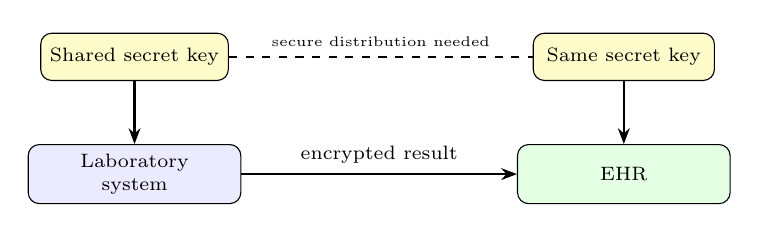
\begin{tikzpicture}[
    node distance=0.9cm,
    box/.style={draw, rounded corners, align=center, minimum width=2.7cm, minimum height=0.75cm, font=\scriptsize},
    key/.style={draw, rounded corners, align=center, fill=yellow!20, minimum width=2.3cm, minimum height=0.6cm, font=\scriptsize},
    link/.style={-{Stealth[length=2mm]}, thick}
]
\node[box, fill=blue!8] (lab) {Laboratory\\system};
\node[box, right=3.5cm of lab, fill=green!10] (ehr) {EHR};
\node[key, above=0.8cm of lab] (k1) {Shared secret key};
\node[key, above=0.8cm of ehr] (k2) {Same secret key};
\draw[link] (lab) -- node[above, font=\scriptsize]{encrypted result} (ehr);
\draw[link] (k1) -- (lab);
\draw[link] (k2) -- (ehr);
\draw[dashed, thick] (k1) -- node[above, font=\tiny]{secure distribution needed} (k2);
\end{tikzpicture}
\end{center}

\begin{block}{Takeaway}
The difficult part is often not encryption itself, but getting the key safely to the right systems.
\end{block}
\end{frame}

\begin{frame}[c]{Cryptanalytic Attacks}
\begin{block}{Concept}
\textbf{Cryptanalysis} tries to exploit weaknesses in the algorithm, message structure, or available
plaintext/ciphertext examples.
\end{block}

\begin{exampleblock}{Hospital example}
If every exported report begins with the same header, a weak encryption mode may reveal patterns
that help an attacker reason about the protected files.
\end{exampleblock}
\end{frame}

\begin{frame}[c]{Brute-Force Attacks}
\begin{block}{Concept}
\textbf{Brute force} tries possible keys until the output looks like meaningful plaintext. Longer keys
make exhaustive search infeasible.
\end{block}

\begin{exampleblock}{Hospital example}
If archived patient files were encrypted with an obsolete short key, an attacker with copied
ciphertext may be able to recover the records later.
\end{exampleblock}
\end{frame}

\begin{frame}[c]{DES and 3DES}
\begin{block}{Historical note}
DES used 64-bit blocks and a 56-bit key. It became insecure against brute force; 3DES applied DES
three times with longer effective keys, but at a performance cost.
\end{block}

\begin{exampleblock}{Hospital example}
Legacy medical devices may still support old cryptographic suites. St. Isidore should identify
where DES or 3DES appears and plan migration.
\end{exampleblock}
\end{frame}

\begin{frame}[c]{How DES Works}
\begin{block}{Mechanism}
DES is a \textbf{Feistel block cipher}. Each 64-bit block is split into left and right halves. In
each round, DES transforms one half with a round key, combines it with the other half using XOR, and
then swaps the halves.
\end{block}

\begin{exampleblock}{Hospital example}
Think of one 8-byte fragment of a lab result. DES does not encrypt it in one step: it repeatedly
mixes part of the fragment with key material so that changing one bit should spread through the
block.
\end{exampleblock}
\end{frame}

\begin{frame}[c]{Scheme: DES Feistel Round}
\begin{center}
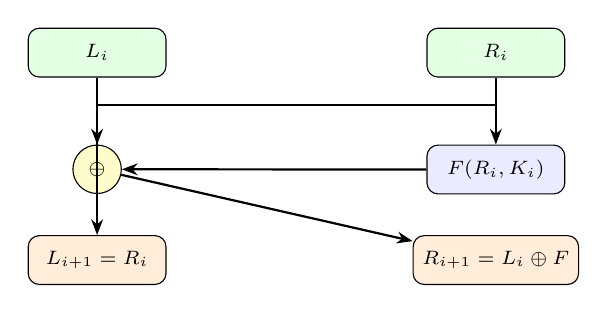
\begin{tikzpicture}[
    node distance=0.65cm,
    box/.style={draw, rounded corners, align=center, minimum width=1.75cm, minimum height=0.62cm, font=\scriptsize},
    op/.style={draw, circle, align=center, minimum size=0.55cm, font=\scriptsize},
    link/.style={-{Stealth[length=2mm]}, thick}
]
\node[box, fill=green!10] (li) {$L_i$};
\node[box, right=3.3cm of li, fill=green!10] (ri) {$R_i$};
\node[box, below=0.85cm of ri, fill=blue!8] (f) {$F(R_i,K_i)$};
\node[op, below=0.85cm of li, fill=yellow!20] (xor) {$\oplus$};
\node[box, below=2.0cm of li, fill=orange!15] (lout) {$L_{i+1}=R_i$};
\node[box, below=2.0cm of ri, fill=orange!15] (rout) {$R_{i+1}=L_i \oplus F$};
\draw[link] (ri) -- (f);
\draw[link] (f.west) -- (xor.east);
\draw[link] (li) -- (xor);
\draw[link] (xor) -- (rout);
\draw[link] (ri.south) -- ++(0,-0.35) -| (lout.north);
\end{tikzpicture}
\end{center}

\begin{block}{Reading the scheme}
The right half becomes the next left half. The next right half is produced by mixing the old left
half with a keyed transformation of the old right half.
\end{block}
\end{frame}

\begin{frame}[c]{Notebook: DES and 3DES}
\begin{block}{Practical example}
Open \texttt{lesson-02/examples/02\_des\_3des\_mechanics.ipynb} after the Feistel round scheme.
\end{block}

\begin{exampleblock}{What students should notice}
The notebook runs real DES-CBC and 3DES, then uses a small toy Feistel network to show why
decryption works by applying round keys in reverse order.
\end{exampleblock}
\end{frame}

\begin{frame}[c]{AES}
\begin{block}{Modern standard}
The Advanced Encryption Standard is a symmetric block cipher with 128-bit blocks and key sizes of
128, 192, or 256 bits \cite{nist_fips_197}.
\end{block}

\begin{exampleblock}{Hospital example}
AES is commonly used to encrypt backups, databases, disks, VPN traffic, and secure application
channels in healthcare environments.
\end{exampleblock}
\end{frame}

\begin{frame}[c]{How AES Works}
\begin{block}{Mechanism}
AES treats each 128-bit block as a 4-by-4 byte matrix called the \textbf{state}. It first mixes in
key material, then repeats a round structure: \textbf{SubBytes}, \textbf{ShiftRows},
\textbf{MixColumns}, and \textbf{AddRoundKey}. The final round omits MixColumns.
\end{block}

\begin{exampleblock}{Hospital example}
For an encrypted backup, AES processes block after block of patient data. A safe mode of operation
also makes sure repeated or changed backup chunks do not create predictable results.
\end{exampleblock}
\end{frame}

\begin{frame}[c]{AES Round Operations}
\begin{block}{Algorithmic view}
\begin{enumerate}
    \item \textbf{SubBytes}: replace each byte through a non-linear lookup table.
    \item \textbf{ShiftRows}: rotate rows so bytes move to new columns.
    \item \textbf{MixColumns}: combine bytes inside each column.
    \item \textbf{AddRoundKey}: XOR the state with round-key bytes.
\end{enumerate}
\end{block}

\begin{exampleblock}{Hospital example}
If one byte changes in a medication record block, the substitutions and mixing spread that change
through the block across later rounds.
\end{exampleblock}
\end{frame}

\begin{frame}[c]{Scheme: AES Round}
\begin{center}
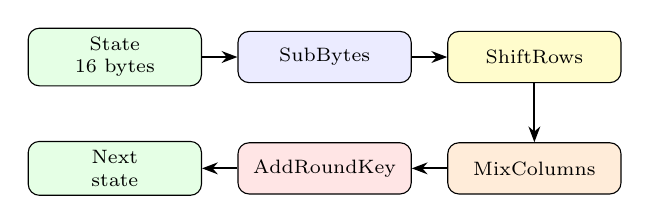
\begin{tikzpicture}[
    node distance=0.45cm,
    aesstep/.style={draw, rounded corners, align=center, minimum width=2.2cm, minimum height=0.65cm, font=\scriptsize},
    link/.style={-{Stealth[length=2mm]}, thick}
]
\node[aesstep, fill=green!10] (state) {State\\16 bytes};
\node[aesstep, right=of state, fill=blue!8] (sub) {SubBytes};
\node[aesstep, right=of sub, fill=yellow!20] (shift) {ShiftRows};
\node[aesstep, below=0.75cm of shift, fill=orange!15] (mix) {MixColumns};
\node[aesstep, left=of mix, fill=red!10] (key) {AddRoundKey};
\node[aesstep, left=of key, fill=green!10] (next) {Next\\state};
\draw[link] (state) -- (sub);
\draw[link] (sub) -- (shift);
\draw[link] (shift) -- (mix);
\draw[link] (mix) -- (key);
\draw[link] (key) -- (next);
\end{tikzpicture}
\end{center}

\begin{block}{Reading the scheme}
AES security comes from repeating simple operations many times with different round keys.
\end{block}
\end{frame}

\begin{frame}[c]{Recap: Symmetric Encryption}
\begin{block}{Takeaways}
\begin{itemize}
    \item Symmetric encryption is fast and widely used.
    \item Security depends on strong algorithms and strong key management.
    \item DES is obsolete; 3DES is legacy; AES is the modern standard.
    \item A block cipher still needs a safe mode when used on real messages.
    \item Key exposure compromises every message protected with that key.
\end{itemize}
\end{block}
\end{frame}

\section{Blocks, Streams, and Modes}
\sectiontitleframe{Blocks, Streams, and Modes}

\begin{frame}[c]{Section Context: Blocks, Streams, and Modes}
\begin{block}{What we are talking about}
Encryption algorithms must process real data: files, messages, streams, and databases. This
section explains why the way data is split and processed matters.
\end{block}

\begin{exampleblock}{Hospital lens}
St. Isidore encrypts long files, short alerts, real-time connections, and database fields. Different
uses require different cryptographic constructions.
\end{exampleblock}
\end{frame}

\begin{frame}[c]{Block Ciphers}
\begin{block}{Concept}
A \textbf{block cipher} encrypts fixed-size blocks of data. AES, for example, uses 128-bit blocks.
\end{block}

\begin{exampleblock}{Hospital example}
An encrypted backup file is divided into many blocks. The mode of operation determines how those
blocks are combined and protected.
\end{exampleblock}
\end{frame}

\begin{frame}[c]{Modes of Operation}
\begin{block}{Concept}
A block cipher such as AES only defines how to encrypt \textbf{one fixed-size block}. A
\textbf{mode of operation} defines how to use that block cipher safely across longer messages.
\end{block}

\begin{exampleblock}{Hospital example}
An EHR backup is much longer than one AES block. The mode decides how each encrypted block relates
to the previous block, to randomness, and sometimes to an authentication tag.
\end{exampleblock}
\end{frame}

\begin{frame}[c]{Electronic Codebook (ECB)}
\begin{block}{Concept}
ECB encrypts equal plaintext blocks into equal ciphertext blocks under the same key. This leaks
patterns and is not suitable for most real-world protection.
\end{block}

\begin{exampleblock}{Hospital example}
If many records start with the same structured header, ECB can reveal that repetition even though
the content is encrypted.
\end{exampleblock}
\end{frame}

\begin{frame}[c]{Scheme: ECB Pattern Leakage}
\begin{center}
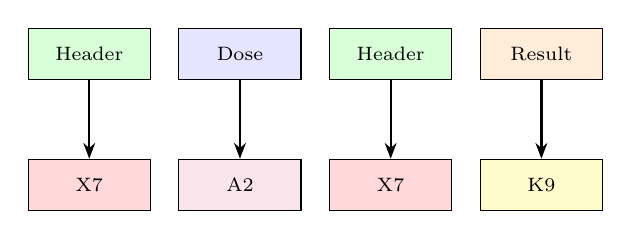
\begin{tikzpicture}[
    node distance=0.35cm,
    block/.style={draw, minimum width=1.55cm, minimum height=0.65cm, align=center, font=\scriptsize},
    link/.style={-{Stealth[length=2mm]}, thick}
]
\node[block, fill=green!15] (p1) {Header};
\node[block, right=of p1, fill=blue!10] (p2) {Dose};
\node[block, right=of p2, fill=green!15] (p3) {Header};
\node[block, right=of p3, fill=orange!15] (p4) {Result};
\node[block, below=1cm of p1, fill=red!15] (c1) {X7};
\node[block, right=of c1, fill=purple!10] (c2) {A2};
\node[block, right=of c2, fill=red!15] (c3) {X7};
\node[block, right=of c3, fill=yellow!20] (c4) {K9};
\draw[link] (p1) -- (c1);
\draw[link] (p2) -- (c2);
\draw[link] (p3) -- (c3);
\draw[link] (p4) -- (c4);
\end{tikzpicture}
\end{center}

\begin{block}{Reading the scheme}
Repeated plaintext blocks produce repeated ciphertext blocks. The attacker sees structure.
\end{block}
\end{frame}

\begin{frame}[c]{CBC and GCM}
\begin{block}{Two safer directions}
\textbf{Cipher Block Chaining (CBC)} uses an initialization vector and chains blocks to hide direct
repetition. \textbf{Galois/Counter Mode (GCM)} is an authenticated-encryption mode: it encrypts data
and computes a tag that detects tampering.
\end{block}

\begin{exampleblock}{Hospital example}
For St. Isidore, CBC can hide repeated backup structure when used correctly, but GCM is preferable
for many messages because changed patient data or metadata will fail authentication.
\end{exampleblock}
\end{frame}

\begin{frame}[c]{Notebook: AES Modes}
\begin{block}{Practical example}
Open the AES modes notebook in \texttt{lesson-02/examples}:\\
\texttt{03\_aes\_modes\_authenticated\_encryption.ipynb}
\end{block}

\begin{exampleblock}{What students should notice}
The notebook shows that AES-ECB leaks repeated blocks, AES-CBC hides those repetitions, and AES-GCM
adds authentication so tampering is detected.
\end{exampleblock}
\end{frame}

\begin{frame}[c]{Stream Ciphers}
\begin{block}{Concept}
A \textbf{stream cipher} generates a keystream and combines it with plaintext, often byte by byte or
bit by bit.
\end{block}

\begin{exampleblock}{Hospital example}
Real-time encrypted communication, such as secure web traffic, may use constructions that behave
like a protected stream rather than a static file encryption process.
\end{exampleblock}
\end{frame}

\begin{frame}[c]{Stream Cipher Safety}
\begin{block}{Key point}
A stream cipher is only safe when the same key stream is not reused. In practice this means
\textbf{never reuse the same key and nonce together}.
\end{block}

\begin{block}{Nonce}
A \textbf{nonce} is a value used once with a key. It does not always need to be secret, but it must
follow the algorithm's uniqueness or randomness requirements.
\end{block}

\begin{exampleblock}{Hospital example}
If two telemetry messages from an infusion pump reuse the same stream, an attacker can compare the
ciphertexts and learn how the clinical messages differ.
\end{exampleblock}

\end{frame}

\begin{frame}[c]{Notebook: Stream Encryption}
\begin{block}{Practical example}
Open \texttt{lesson-02/examples/04\_stream\_cipher\_chacha20.ipynb} after the stream cipher safety
slide.
\end{block}

\begin{exampleblock}{What students should notice}
The notebook encrypts telemetry-like messages with ChaCha20 and then deliberately reuses a nonce.
The XOR of ciphertexts reveals the XOR of plaintexts.
\end{exampleblock}
\end{frame}

\begin{frame}[c]{Block vs Stream Uses}
\begin{center}
\scriptsize
\renewcommand{\arraystretch}{1.25}
\begin{tabular}{>{\bfseries}p{0.27\textwidth} p{0.28\textwidth} p{0.32\textwidth}}
\toprule
Approach & Typical strength & Hospital examples \\
\midrule
Block cipher & Good for structured data and files when used with safe modes & Backups, databases, file transfers \\
Stream cipher & Good for continuous communication when nonces and keystreams are safe & Secure channels, web sessions, VPN traffic \\
\bottomrule
\end{tabular}
\end{center}

\begin{block}{Important}
Both approaches can be secure or insecure depending on the algorithm, mode, keys, nonces, and
implementation.
\end{block}
\end{frame}

\begin{frame}[c]{Recap: Blocks, Streams, and Modes}
\begin{block}{Takeaways}
\begin{itemize}
    \item Block ciphers process fixed-size blocks.
    \item Stream ciphers protect data as a continuous flow.
    \item ECB is dangerous because it leaks repetition.
    \item Correct modes, nonces, and implementation details are part of security.
\end{itemize}
\end{block}
\end{frame}

\section{Authentication and Hashes}
\sectiontitleframe{Authentication and Hashes}

\begin{frame}[c]{Section Context: Authentication and Hashes}
\begin{block}{What we are talking about}
Encryption protects confidentiality, but active attacks require integrity and authentication.
This section explains MACs and hash functions.
\end{block}

\begin{exampleblock}{Hospital lens}
When a pharmacy order arrives, the hospital must know not only that it was private, but also that
it is genuine, unchanged, recent, and in the right sequence.
\end{exampleblock}
\end{frame}

\begin{frame}[c]{Message Authentication}
\begin{block}{Concept}
A message is authentic when the receiver can verify its source and detect changes to its content.
Good authentication can also check sequence and freshness.
\end{block}

\begin{exampleblock}{Hospital example}
The EHR should reject a lab result if it was modified, replayed from yesterday, or sent by a system
pretending to be the laboratory.
\end{exampleblock}
\end{frame}

\begin{frame}[c]{Why Encryption Alone Is Not Enough}
\begin{block}{Concept}
Confidentiality does not automatically imply integrity. Some encrypted data can still be reordered,
replayed, or tampered with unless authentication is included.
\end{block}

\begin{exampleblock}{Hospital example}
If encrypted medication-order blocks can be rearranged without detection, the receiver may decrypt
valid-looking but clinically wrong content.
\end{exampleblock}
\end{frame}

\begin{frame}[c]{Message Authentication Code}
\begin{block}{Concept}
A \textbf{Message Authentication Code} (MAC) is a short tag computed from a message and a shared
secret key. The receiver recomputes the tag and compares it.
\end{block}

\begin{exampleblock}{Hospital example}
The lab system attaches a MAC to each result message. The EHR verifies the MAC before accepting
the result into the patient record.
\end{exampleblock}
\end{frame}

\begin{frame}[c]{Scheme: MAC Verification}
\begin{center}
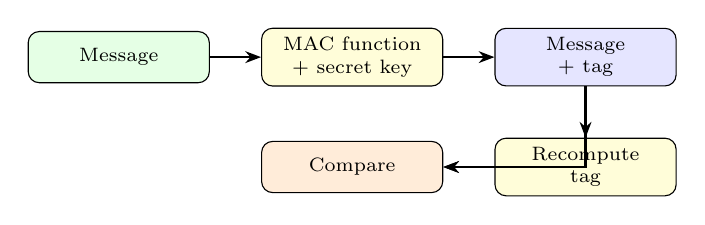
\begin{tikzpicture}[
    node distance=0.65cm,
    box/.style={draw, rounded corners, align=center, minimum width=2.3cm, minimum height=0.65cm, font=\scriptsize},
    link/.style={-{Stealth[length=2mm]}, thick}
]
\node[box, fill=green!10] (msg) {Message};
\node[box, right=of msg, fill=yellow!15] (mac1) {MAC function\\+ secret key};
\node[box, right=of mac1, fill=blue!10] (send) {Message\\+ tag};
\node[box, below=of send, fill=yellow!15] (mac2) {Recompute\\tag};
\node[box, left=of mac2, fill=orange!15] (cmp) {Compare};
\draw[link] (msg) -- (mac1);
\draw[link] (mac1) -- (send);
\draw[link] (send) -- (mac2);
\draw[link] (mac2) -- (cmp);
\draw[link] (send) |- (cmp);
\end{tikzpicture}
\end{center}

\begin{block}{Takeaway}
If the tags match, the receiver gains confidence that the message came from someone with the key
and was not altered.
\end{block}
\end{frame}

\begin{frame}[c]{Hash Functions}
\begin{block}{Concept}
A \textbf{hash function} maps data of variable length to a fixed-length digest. A secure hash acts
like a fingerprint of the input.
\end{block}

\begin{exampleblock}{Hospital example}
The hospital computes a hash of a software update before installation. If the downloaded file has
changed, the hash will not match the expected value.
\end{exampleblock}
\end{frame}

\begin{frame}[c]{Properties of Secure Hashes}
\begin{itemize}
    \item \textbf{Preimage resistance}: given a digest, it is infeasible to find a matching input.
    \item \textbf{Second-preimage resistance}: given one input, it is infeasible to find a different input with the same digest.
    \item \textbf{Collision resistance}: it is infeasible to find any two different inputs with the same digest.
\end{itemize}

\begin{exampleblock}{Hospital example}
These properties help protect password storage, file-integrity monitoring, and digital signatures.
\end{exampleblock}
\end{frame}

\begin{frame}[c]{Hashing Passwords}
\begin{block}{Concept}
Systems should store password verifiers, not plaintext passwords. In practice this requires
password-hashing schemes with salts and work factors, not a bare fast hash.
\end{block}

\begin{exampleblock}{Hospital example}
If an attacker steals the staff account database, salted password hashes make password recovery
harder than if plaintext passwords were stored.
\end{exampleblock}
\end{frame}

\begin{frame}[c]{File Integrity Monitoring}
\begin{block}{Concept}
Hash values can help detect whether important files changed. The reference hashes must be
protected from attackers.
\end{block}

\begin{exampleblock}{Hospital example}
St. Isidore stores trusted hashes of critical EHR configuration files. A nightly check alerts IT if
malware modifies them.
\end{exampleblock}
\end{frame}

\begin{frame}[c]{SHA}
\begin{block}{Standard family}
The Secure Hash Standard defines SHA algorithms used in many security applications
\cite{nist_fips_180_4}. Algorithm choice matters because older hashes may become weak over time.
\end{block}

\begin{exampleblock}{Hospital example}
The hospital prefers modern SHA-2 or SHA-3 based mechanisms where appropriate, and avoids legacy
uses of broken hashes in certificates or signatures.
\end{exampleblock}
\end{frame}

\begin{frame}[c]{How SHA Works}
\begin{block}{Algorithm idea}
SHA algorithms process data in blocks. Each block updates an internal state through many rounds of
bit operations. At the end, the final state becomes the fixed-length \textbf{digest}.
\end{block}

\begin{exampleblock}{Hospital example}
If a radiology report changes from ``no fracture'' to ``fracture'', SHA-256 produces a completely
different digest. The digest does not hide the report; it detects whether the exact bytes changed.
\end{exampleblock}
\end{frame}

\begin{frame}[c]{Scheme: SHA Digest}
\begin{center}
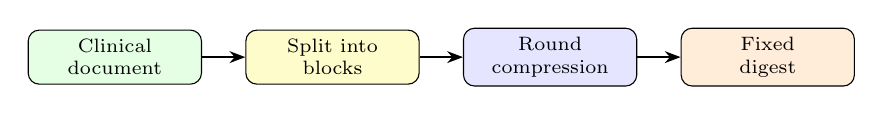
\begin{tikzpicture}[
    node distance=0.55cm,
    box/.style={draw, rounded corners, align=center, minimum width=2.2cm, minimum height=0.62cm, font=\scriptsize},
    link/.style={-{Stealth[length=2mm]}, thick}
]
\node[box, fill=green!10] (msg) {Clinical\\document};
\node[box, right=of msg, fill=yellow!20] (blocks) {Split into\\blocks};
\node[box, right=of blocks, fill=blue!10] (compress) {Round\\compression};
\node[box, right=of compress, fill=orange!15] (digest) {Fixed\\digest};
\draw[link] (msg) -- (blocks);
\draw[link] (blocks) -- (compress);
\draw[link] (compress) -- (digest);
\end{tikzpicture}
\end{center}

\begin{block}{Important}
SHA is \textbf{not encryption}: there is no decryption key and no way to recover the original
message from the digest.
\end{block}
\end{frame}

\begin{frame}[c]{Notebook: Hashes, HMAC, and Passwords}
\begin{block}{Practical example}
Open \texttt{lesson-02/examples/05\_hashes\_hmac\_passwords.ipynb} after the SHA slide.
\end{block}

\begin{exampleblock}{What students should notice}
The notebook compares file hashes, verifies an HMAC on a lab message, and derives a salted password
verifier. The same digest idea appears in different security roles.
\end{exampleblock}
\end{frame}

\begin{frame}[c]{Recap: Authentication and Hashes}
\begin{block}{Takeaways}
\begin{itemize}
    \item Encryption alone does not fully protect against active attacks.
    \item MACs authenticate messages using a shared secret key.
    \item Hash functions provide fixed-length fingerprints of data.
    \item Secure hashes support passwords, file checks, MACs, and digital signatures.
\end{itemize}
\end{block}
\end{frame}

\section{Public-Key Cryptography}
\sectiontitleframe{Public-Key Cryptography}

\begin{frame}[c]{Section Context: Public-Key Cryptography}
\begin{block}{What we are talking about}
Public-key cryptography uses a pair of keys: one public and one private. It changes how systems
solve confidentiality, authentication, signatures, and key distribution.
\end{block}

\begin{exampleblock}{Hospital lens}
St. Isidore uses public-key cryptography when browsers validate the patient portal certificate,
when VPN sessions establish keys, and when signed software updates are verified.
\end{exampleblock}
\end{frame}

\begin{frame}[c]{Asymmetric Keys}
\begin{block}{Concept}
Each participant has a \textbf{public key} that can be shared and a \textbf{private key} that must stay
secret. What one key does, the paired key can verify or reverse, depending on the scheme.
\end{block}

\begin{exampleblock}{Hospital example}
The patient portal publishes a certificate containing its public key. The matching private key
stays protected on the server or in a hardware security module.
\end{exampleblock}
\end{frame}

\begin{frame}[c]{Confidentiality with Public Keys}
\begin{block}{Concept}
To send confidential data to Alice, Bob encrypts using Alice's public key. Only Alice's private key
can decrypt.
\end{block}

\begin{exampleblock}{Hospital example}
An external clinic can encrypt a referral package so that only St. Isidore's receiving service can
open it.
\end{exampleblock}
\end{frame}

\begin{frame}[c]{Authentication with Private Keys}
\begin{block}{Concept}
To prove origin, Bob signs with his private key. Anyone with Bob's public key can verify that the
signature matches.
\end{block}

\begin{exampleblock}{Hospital example}
A signed software update proves that the update came from the trusted vendor and was not modified
after signing.
\end{exampleblock}
\end{frame}

\begin{frame}[c]{Scheme: Public-Key Uses}
\begin{center}
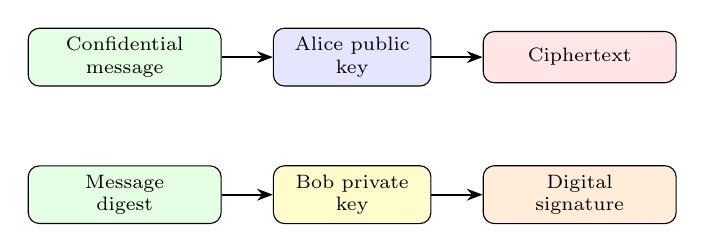
\begin{tikzpicture}[
    node distance=0.65cm,
    box/.style={draw, rounded corners, align=center, minimum width=2.45cm, minimum height=0.65cm, font=\scriptsize},
    key/.style={draw, rounded corners, align=center, minimum width=2.0cm, minimum height=0.55cm, font=\scriptsize},
    link/.style={-{Stealth[length=2mm]}, thick}
]
\node[box, fill=green!10] (msg1) {Confidential\\message};
\node[key, right=of msg1, fill=blue!10] (pubA) {Alice public\\key};
\node[box, right=of pubA, fill=red!10] (ct) {Ciphertext};
\draw[link] (msg1) -- (pubA);
\draw[link] (pubA) -- (ct);
\node[box, below=1.0cm of msg1, fill=green!10] (msg2) {Message\\digest};
\node[key, right=of msg2, fill=yellow!20] (privB) {Bob private\\key};
\node[box, right=of privB, fill=orange!15] (sig) {Digital\\signature};
\draw[link] (msg2) -- (privB);
\draw[link] (privB) -- (sig);
\end{tikzpicture}
\end{center}

\begin{block}{Reading the scheme}
Public-key encryption and digital signatures use key pairs differently. The goal determines which
key is used.
\end{block}
\end{frame}

\begin{frame}[c]{Families of Public-Key Algorithms}
\begin{block}{What changes between algorithms}
Public-key algorithms are not interchangeable names. Each family is built around a hard mathematical
problem and is usually designed for one main purpose: \textbf{encryption}, \textbf{digital
signature}, or \textbf{key agreement}.
\end{block}

\begin{exampleblock}{Hospital example}
The patient portal certificate may use one algorithm to sign its identity, while the VPN handshake
uses another algorithm to agree on fresh session keys. Both are public-key cryptography, but they do
different jobs.
\end{exampleblock}
\end{frame}

\begin{frame}[c]{RSA: Trapdoor Computation}
\begin{block}{Algorithm idea}
RSA is based on modular arithmetic with a public modulus. The public key can transform data in one
direction, while the private key provides the \textbf{trapdoor} needed to reverse or sign that
transformation.
\end{block}

\begin{exampleblock}{Hospital example}
An external clinic can encrypt a small session key with St. Isidore's RSA public key. Only the
hospital private key can unwrap it. The same RSA key family can also sign messages when used with a
signature padding scheme.
\end{exampleblock}
\end{frame}

\begin{frame}[c]{RSA in Practice}
\begin{block}{Important distinction}
RSA should not be used to encrypt large clinical files directly. It is usually used to protect
small values, such as a symmetric session key, or to create digital signatures.
\end{block}

\begin{exampleblock}{Hospital example}
For an imaging report, St. Isidore encrypts the file with AES, then uses RSA only to protect the
AES key. This is the digital-envelope pattern used later in the lesson.
\end{exampleblock}
\end{frame}

\begin{frame}[c]{Diffie-Hellman Key Agreement}
\begin{block}{Concept}
Diffie-Hellman allows two parties to establish a shared secret over an insecure channel
\cite{diffie_hellman_1976}. By itself, basic Diffie-Hellman does not authenticate who is on the
other side.
\end{block}

\begin{exampleblock}{Hospital example}
A doctor connects to the VPN from home. The protocol can agree on session keys, but certificates
and authentication are needed to prevent an attacker from impersonating the hospital.
\end{exampleblock}
\end{frame}

\begin{frame}[c]{How Diffie-Hellman Works}
\begin{block}{Algorithm idea}
Each side creates a private random value and publishes a related public value. The two public values
can be exchanged openly. Combining \textbf{my private value} with \textbf{your public value} gives
the same shared secret on both sides.
\end{block}

\begin{exampleblock}{Hospital example}
The doctor's laptop and the VPN gateway exchange public handshake values. An observer can see those
values, but cannot feasibly compute the final session key without one of the private values.
\end{exampleblock}
\end{frame}

\begin{frame}[c]{Scheme: Diffie-Hellman}
\begin{center}
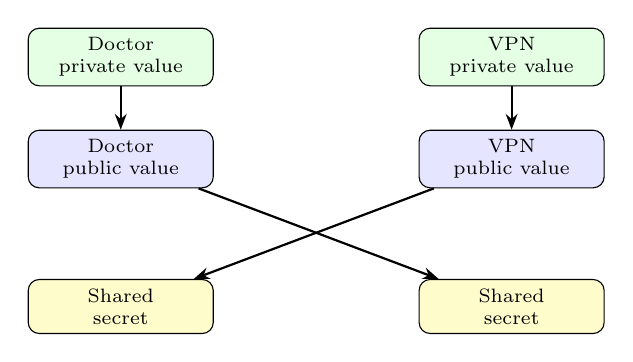
\begin{tikzpicture}[
    node distance=0.55cm,
    box/.style={draw, rounded corners, align=center, minimum width=2.35cm, minimum height=0.62cm, font=\scriptsize},
    link/.style={-{Stealth[length=2mm]}, thick}
]
\node[box, fill=green!10] (docpriv) {Doctor\\private value};
\node[box, below=of docpriv, fill=blue!10] (docpub) {Doctor\\public value};
\node[box, right=2.6cm of docpriv, fill=green!10] (vpnpriv) {VPN\\private value};
\node[box, below=of vpnpriv, fill=blue!10] (vpnpub) {VPN\\public value};
\node[box, below=1.15cm of docpub, fill=yellow!20] (docsecret) {Shared\\secret};
\node[box, below=1.15cm of vpnpub, fill=yellow!20] (vpnsecret) {Shared\\secret};
\draw[link] (docpriv) -- (docpub);
\draw[link] (vpnpriv) -- (vpnpub);
\draw[link] (docpub) -- (vpnsecret);
\draw[link] (vpnpub) -- (docsecret);
\end{tikzpicture}
\end{center}

\begin{block}{Reading the scheme}
The shared secret is not transmitted. Each side derives it locally from one private value and one
received public value.
\end{block}
\end{frame}

\begin{frame}[c]{Notebook: Diffie-Hellman}
\begin{block}{Practical example}
Open \texttt{lesson-02/examples/07\_diffie\_hellman\_randomness.ipynb} after the Diffie-Hellman
slide, then return to it again in the randomness section.
\end{block}

\begin{exampleblock}{What students should notice}
The doctor and the hospital compute the same shared secret without sending that secret over the
network. The notebook then derives a session key from it.
\end{exampleblock}
\end{frame}

\begin{frame}[c]{DSS and DSA: Signature Only}
\begin{block}{Algorithm idea}
The Digital Signature Standard (DSS) defines approved ways to create digital signatures. DSA is a
signature algorithm from that family. It does \textbf{not} encrypt data and it does \textbf{not}
establish shared keys.
\end{block}

\begin{exampleblock}{Hospital example}
A software vendor can sign a pacemaker gateway firmware update. The hospital verifies the signature
before installation, but the signature itself does not hide the update contents.
\end{exampleblock}
\end{frame}

\begin{frame}[c]{How DSA Is Used}
\begin{block}{Signing flow}
DSA signs a \textbf{hash} of the message, not the whole message directly. The private key creates a
signature value; the public key verifies whether that signature matches the message hash.
\end{block}

\begin{exampleblock}{Hospital example}
The vendor signs the hash of a firmware package. St. Isidore hashes the downloaded package again
and verifies the signature with the vendor public key before installing it.
\end{exampleblock}
\end{frame}

\begin{frame}[c]{Scheme: DSA Signature}
\begin{center}
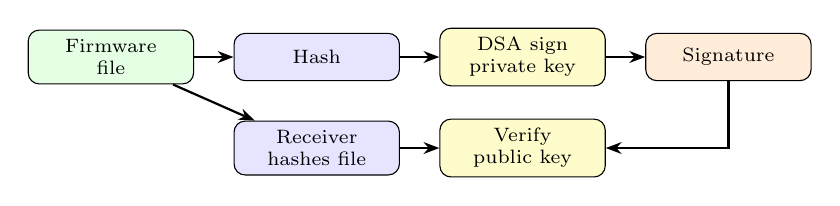
\begin{tikzpicture}[
    node distance=0.5cm,
    box/.style={draw, rounded corners, align=center, minimum width=2.1cm, minimum height=0.6cm, font=\scriptsize},
    link/.style={-{Stealth[length=2mm]}, thick}
]
\node[box, fill=green!10] (msg) {Firmware\\file};
\node[box, right=of msg, fill=blue!10] (hash) {Hash};
\node[box, right=of hash, fill=yellow!20] (sign) {DSA sign\\private key};
\node[box, right=of sign, fill=orange!15] (sig) {Signature};
\node[box, below=of hash, fill=blue!10] (hash2) {Receiver\\hashes file};
\node[box, right=of hash2, fill=yellow!20] (verify) {Verify\\public key};
\draw[link] (msg) -- (hash);
\draw[link] (hash) -- (sign);
\draw[link] (sign) -- (sig);
\draw[link] (msg) -- (hash2);
\draw[link] (sig) |- (verify);
\draw[link] (hash2) -- (verify);
\end{tikzpicture}
\end{center}

\begin{block}{Takeaway}
DSA gives authenticity and integrity, but not confidentiality.
\end{block}
\end{frame}

\begin{frame}[c]{Algorithm Families: Recap Map}
\begin{center}
\scriptsize
\renewcommand{\arraystretch}{1.25}
\begin{tabular}{>{\bfseries}p{0.24\textwidth} p{0.2\textwidth} p{0.2\textwidth} p{0.22\textwidth}}
\toprule
Algorithm family & Digital signature & Key agreement & Encryption \\
\midrule
RSA & Yes & Legacy key transport & Yes, for small values \\
Diffie-Hellman & No & Yes & No \\
DSS / DSA & Yes & No & No \\
\bottomrule
\end{tabular}
\end{center}

\begin{block}{Important}
Modern protocols combine these families with symmetric encryption. The public-key step establishes
identity or keys; AES-like symmetric encryption protects the bulk data.
\end{block}
\end{frame}

\begin{frame}[c]{Recap: Public-Key Cryptography}
\begin{block}{Takeaways}
\begin{itemize}
    \item Public-key cryptography uses key pairs, not one shared secret.
    \item Public keys can be shared; private keys must be protected.
    \item It supports encryption, signatures, and key establishment.
    \item It usually works together with symmetric encryption in real systems.
\end{itemize}
\end{block}
\end{frame}

\section{Signatures, Certificates, and Envelopes}
\sectiontitleframe{Signatures, Certificates, and Envelopes}

\begin{frame}[c]{Section Context: Signatures, Certificates, and Envelopes}
\begin{block}{What we are talking about}
Public keys are useful only when we can trust whose key they are. This section connects digital
signatures, certificates, certificate authorities, and hybrid encryption.
\end{block}

\begin{exampleblock}{Hospital lens}
The hospital must trust that the patient portal certificate belongs to St. Isidore, that vendor
updates are signed by the vendor, and that encrypted messages reach the intended recipient.
\end{exampleblock}
\end{frame}

\begin{frame}[c]{Digital Signatures}
\begin{block}{Concept}
A digital signature is usually created by hashing a message and signing the hash with the sender's
private key.
\end{block}

\begin{exampleblock}{Hospital example}
The pharmacy service signs a formulary update. The EHR verifies the signature before using the new
medication rules.
\end{exampleblock}
\end{frame}

\begin{frame}[c]{Scheme: Digital Signature}
\begin{center}
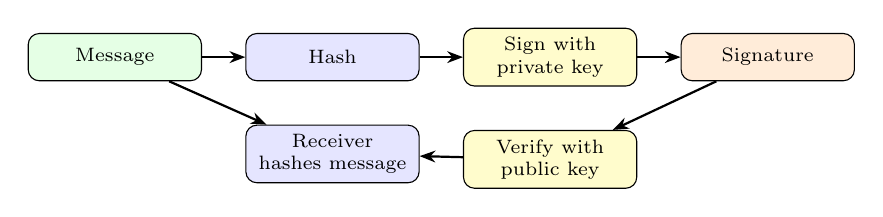
\begin{tikzpicture}[
    node distance=0.55cm,
    box/.style={draw, rounded corners, align=center, minimum width=2.2cm, minimum height=0.6cm, font=\scriptsize},
    link/.style={-{Stealth[length=2mm]}, thick}
]
\node[box, fill=green!10] (msg) {Message};
\node[box, right=of msg, fill=blue!10] (hash) {Hash};
\node[box, right=of hash, fill=yellow!20] (sign) {Sign with\\private key};
\node[box, right=of sign, fill=orange!15] (sig) {Signature};
\node[box, below=of hash, fill=blue!10] (verifyhash) {Receiver\\hashes message};
\node[box, below=of sign, fill=yellow!20] (verify) {Verify with\\public key};
\draw[link] (msg) -- (hash);
\draw[link] (hash) -- (sign);
\draw[link] (sign) -- (sig);
\draw[link] (msg) -- (verifyhash);
\draw[link] (sig) -- (verify);
\draw[link] (verify) -- (verifyhash);
\end{tikzpicture}
\end{center}

\begin{block}{Takeaway}
Signatures provide origin authentication and integrity, but not confidentiality by themselves.
\end{block}
\end{frame}

\begin{frame}[c]{Certificates}
\begin{block}{Concept}
A certificate binds a public key to an identity and is signed by a trusted certificate authority.
It includes identity information, the public key, issuer information, and validity period.
\end{block}

\begin{exampleblock}{Hospital example}
When a patient opens the portal, the browser checks that the portal certificate is valid and issued
for the correct hospital domain.
\end{exampleblock}
\end{frame}

\begin{frame}[c]{Why Certificates Are Needed}
\begin{block}{Threat}
Without certificates, an attacker could publish a fake public key and pretend to be the hospital,
a doctor, or a vendor.
\end{block}

\begin{exampleblock}{Hospital example}
If a fake portal key is accepted, patients may encrypt login credentials and health messages for
the attacker instead of St. Isidore.
\end{exampleblock}
\end{frame}

\begin{frame}[c]{Digital Envelopes}
\begin{block}{Concept}
A \textbf{digital envelope} combines symmetric and public-key cryptography: encrypt the message with
a fresh symmetric key, then encrypt that key with the recipient's public key.
\end{block}

\begin{exampleblock}{Hospital example}
The hospital sends a large imaging report to an external specialist. The file is encrypted with a
fast session key; the session key is protected with the specialist's certified public key.
\end{exampleblock}
\end{frame}

\begin{frame}[c]{Scheme: Digital Envelope}
\begin{center}
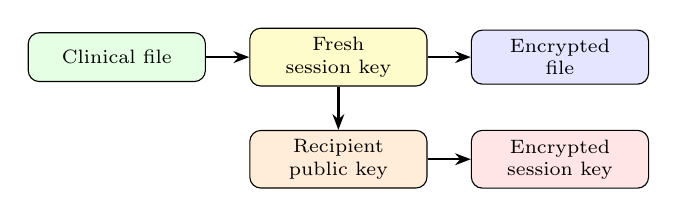
\begin{tikzpicture}[
    node distance=0.55cm,
    box/.style={draw, rounded corners, align=center, minimum width=2.25cm, minimum height=0.62cm, font=\scriptsize},
    link/.style={-{Stealth[length=2mm]}, thick}
]
\node[box, fill=green!10] (msg) {Clinical file};
\node[box, right=of msg, fill=yellow!20] (sk) {Fresh\\session key};
\node[box, right=of sk, fill=blue!10] (encmsg) {Encrypted\\file};
\node[box, below=of sk, fill=orange!15] (pub) {Recipient\\public key};
\node[box, right=of pub, fill=red!10] (enckey) {Encrypted\\session key};
\draw[link] (msg) -- (sk);
\draw[link] (sk) -- (encmsg);
\draw[link] (sk) -- (pub);
\draw[link] (pub) -- (enckey);
\end{tikzpicture}
\end{center}

\begin{block}{Reading the scheme}
Hybrid encryption is efficient: symmetric cryptography protects the data; public-key cryptography
protects the temporary key.
\end{block}
\end{frame}

\begin{frame}[c]{Notebook: RSA and Digital Envelopes}
\begin{block}{Practical example}
Open \texttt{lesson-02/examples/06\_rsa\_signatures\_digital\_envelopes.ipynb} after the digital
envelope scheme.
\end{block}

\begin{exampleblock}{What students should notice}
The notebook signs a prescription approval with RSA, then encrypts a clinical file with a fresh AES
key and wraps that key with the recipient's RSA public key.
\end{exampleblock}
\end{frame}

\begin{frame}[c]{Recap: Signatures, Certificates, and Envelopes}
\begin{block}{Takeaways}
\begin{itemize}
    \item Digital signatures authenticate origin and detect modification.
    \item Certificates bind public keys to identities.
    \item Certificate authorities make public-key trust scalable.
    \item Digital envelopes combine efficient symmetric encryption with public-key key protection.
\end{itemize}
\end{block}
\end{frame}

\section{Keys and Randomness}
\sectiontitleframe{Keys and Randomness}

\begin{frame}[c]{Section Context: Keys and Randomness}
\begin{block}{What we are talking about}
Cryptography depends on keys and unpredictable values. Strong algorithms fail if keys are leaked,
reused incorrectly, generated weakly, or never rotated.
\end{block}

\begin{exampleblock}{Hospital lens}
St. Isidore needs keys for backups, VPN sessions, portal certificates, signed updates, disk
encryption, and secure device communication.
\end{exampleblock}
\end{frame}

\begin{frame}[c]{Key Management}
\begin{block}{Concept}
Key management covers generation, distribution, storage, use, rotation, backup, revocation, and
destruction of cryptographic keys \cite{nist_sp_800_57}.
\end{block}

\begin{exampleblock}{Hospital example}
If the backup encryption key is lost, recovery fails. If the key is stolen, confidentiality fails.
Both availability and confidentiality depend on key management.
\end{exampleblock}
\end{frame}

\begin{frame}[c]{Random Numbers in Cryptography}
\begin{block}{Concept}
Randomness is used for key generation, session keys, stream ciphers, nonces, handshakes, and
replay prevention.
\end{block}

\begin{exampleblock}{Hospital example}
When a clinician opens an HTTPS session with the EHR, random values help create fresh session keys
and prevent reuse of old traffic.
\end{exampleblock}
\end{frame}

\begin{frame}[c]{Uniformity and Independence}
\begin{block}{Concept}
A random sequence should have a roughly uniform distribution and should not allow one value to be
predicted from previous values.
\end{block}

\begin{exampleblock}{Hospital example}
If a medical device generates predictable session keys after reboot, an attacker who observes one
session may predict the next one.
\end{exampleblock}
\end{frame}

\begin{frame}[c]{TRNG and PRNG}
\begin{block}{Concept}
A \textbf{true random number generator} uses a non-deterministic physical source. A
\textbf{pseudorandom generator} is deterministic but can be suitable when properly designed and
seeded.
\end{block}

\begin{exampleblock}{Hospital example}
A secure server may seed a cryptographic PRNG from hardware randomness, then use it to generate
TLS session keys for many portal connections.
\end{exampleblock}
\end{frame}

\begin{frame}[c]{CSPRNG}
\begin{block}{Concept}
A \textbf{cryptographically secure pseudorandom number generator (CSPRNG)} is a PRNG designed so
that observing previous outputs does not make future outputs feasible to predict.
\end{block}

\begin{exampleblock}{Hospital example}
The patient portal should use a CSPRNG for session identifiers, reset tokens, and cryptographic
nonces. A normal simulation-oriented generator is not enough.
\end{exampleblock}
\end{frame}

\begin{frame}[c]{Scheme: Cryptographic Randomness}
\begin{center}
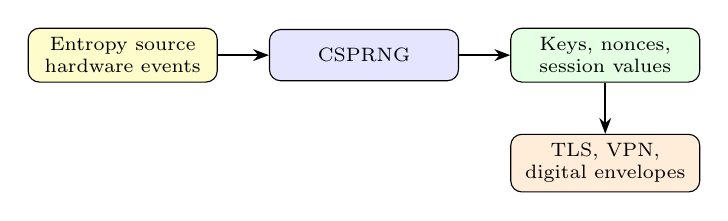
\begin{tikzpicture}[
    node distance=0.65cm,
    box/.style={draw, rounded corners, align=center, minimum width=2.4cm, minimum height=0.65cm, font=\scriptsize},
    link/.style={-{Stealth[length=2mm]}, thick}
]
\node[box, fill=yellow!20] (entropy) {Entropy source\\hardware events};
\node[box, right=of entropy, fill=blue!10] (prng) {CSPRNG};
\node[box, right=of prng, fill=green!10] (keys) {Keys, nonces,\\session values};
\node[box, below=of keys, fill=orange!15] (protocols) {TLS, VPN,\\digital envelopes};
\draw[link] (entropy) -- (prng);
\draw[link] (prng) -- (keys);
\draw[link] (keys) -- (protocols);
\end{tikzpicture}
\end{center}

\begin{block}{Takeaway}
Predictable randomness can silently break otherwise strong cryptography.
\end{block}
\end{frame}

\begin{frame}[c]{Notebook: Randomness}
\begin{block}{Practical example}
Reopen \texttt{lesson-02/examples/07\_diffie\_hellman\_randomness.ipynb} after the randomness
scheme.
\end{block}

\begin{exampleblock}{What students should notice}
The notebook contrasts cryptographic randomness with a deterministic seeded generator. Predictable
values repeat; secure tokens do not.
\end{exampleblock}
\end{frame}

\begin{frame}[c]{TLS as a Preview}
\begin{block}{Connection}
TLS combines many ideas from this lesson: certificates, public-key authentication, key agreement,
symmetric encryption, MACs or authenticated encryption, and fresh random values \cite{rfc8446}.
\end{block}

\begin{exampleblock}{Hospital example}
When patients use the portal, TLS helps them verify the hospital site, protects credentials in
transit, and creates fresh keys for the session.
\end{exampleblock}
\end{frame}

\begin{frame}[c]{Recap: Keys and Randomness}
\begin{block}{Takeaways}
\begin{itemize}
    \item Key management is part of cryptographic security, not an administrative afterthought.
    \item Randomness supports keys, nonces, session setup, and replay protection.
    \item PRNGs must be cryptographically strong and properly seeded.
    \item TLS shows how encryption concepts combine in real network security.
\end{itemize}
\end{block}
\end{frame}

\section{Putting It Together}

\begin{frame}[c]{Connecting the Concepts}
\begin{block}{The full picture}
Encryption protects confidentiality, but healthcare security also needs authentication, integrity,
key management, certificates, and operational procedures.
\end{block}

\begin{exampleblock}{St. Isidore Hospital}
A secure lab-result workflow may use TLS for transport, certificates for server identity, symmetric
session keys for speed, message authentication for integrity, and logs for accountability.
\end{exampleblock}
\end{frame}

\begin{frame}[c]{What Encryption Does Not Solve}
\begin{block}{Important boundary}
Encryption does not fix weak access control, stolen endpoints, bad workflows, missing backups, or
users who are tricked into approving the wrong action.
\end{block}

\begin{exampleblock}{Hospital example}
If an attacker logs in as a real clinician, encryption may protect the network path while the EHR
still reveals records to the compromised account.
\end{exampleblock}
\end{frame}

\begin{frame}[c]{Bridge to Later Lessons}
\begin{block}{What comes next}
Later lessons will place these mechanisms inside real systems and regulations.
\end{block}

\begin{itemize}
    \item \textbf{Basic networking}: where TLS, VPNs, and encrypted channels sit.
    \item \textbf{Access management}: who can use keys and decrypt data.
    \item \textbf{GDPR}: why encryption, pseudonymisation, and breach risk matter for personal data.
    \item \textbf{Operations}: how keys, certificates, backups, and incidents are managed.
\end{itemize}
\end{frame}

\begin{frame}[c]{Doubts? Mail me!}
\begin{center}
\Large g.pisano@unibo.it
\end{center}
\end{frame}

\begin{frame}[allowframebreaks]
\titlepage
\end{frame}

%===============================================================================
\section*{\refname}
%===============================================================================

\setbeamertemplate{page number in head/foot}{}
%/////////
\begin{frame}[c,allowframebreaks,noframenumbering]{\refname}
%\begin{frame}[t,allowframebreaks,noframenumbering]{\refname}
%	\tiny
	\scriptsize
%	\footnotesize
	\bibliographystyle{apalike-AMS}
	\bibliography{main}
\end{frame}

\end{document}
